\documentclass[a4paper]{article}

\usepackage[14pt]{extsizes} % чтобы использовать шрифт размером больше 12
\usepackage{cmap} % для кодировки шрифтов в pdf
\usepackage[T2A]{fontenc} % пакет указывает внутреннюю кодировку в системе LaTeX
\usepackage[utf8]{inputenc} % кодировка  
\usepackage[english, russian]{babel} % пакет для локализации

\usepackage{graphicx} % для вставки картинок
\usepackage{amssymb,amsfonts,amsmath,amsthm} % математические дополнения от АМС
\usepackage{indentfirst} % отделять первую строку раздела абзацным отступом тоже
\usepackage{makecell} % для создания таблиц
\usepackage{multirow} % для продвинутых таблиц
\usepackage{setspace} % для изменения междустрочного интервала
\usepackage{ulem} % подчеркивания

\usepackage[left=20mm, top=15mm, right=15mm, bottom=15mm, nohead, footskip=10mm]{geometry} % настройки полей документа

\linespread{1.3} % полуторный интервал
 
\begin{document} % начало документа
 
% НАЧАЛО ТИТУЛЬНОГО ЛИСТА

\begin{titlepage}
\noindent
\begin{minipage}{0.05\textwidth}

\includegraphics[scale=0.4]{img/01.png}
\end{minipage}
\hfill
\begin{minipage}{0.85\textwidth}
\raggedleft

\begin{center}
\fontsize{12pt}{0.3\baselineskip}\selectfont \textbf{Министерство науки и высшего образования Российской Федерации \\ Федеральное государственное бюджетное образовательное учреждение \\ высшего образования \\ <<Московский государственный технический университет \\ имени Н.Э. Баумана \\ (национальный исследовательский университет)>> \\ (МГТУ им. Н.Э. Баумана)}
\end{center}
\end{minipage}

\begin{center}
\fontsize{12pt}{0.1\baselineskip}\selectfont
\noindent\makebox[\linewidth]{\rule{\textwidth}{4pt}} \makebox[\linewidth]{\rule{\textwidth}{1pt}}
\end{center}

\begin{flushleft}
\fontsize{12pt}{0.8\baselineskip}
\selectfont
ФАКУЛЬТЕТ \uline{<<\textbf{Фундаментальные науки}>>}
			
КАФЕДРА \hspace{4mm} \uline{<<\textbf{Прикладная математика}>>}
\end{flushleft}

\vspace{3mm}

\begin{center}
	\begin{large}
		\textbf{РЕФЕРАТ \\ ПО ПРЕДМЕТУ:}
	\end{large}
\end{center}

\begin{center}
\begin{large}		
\uline{\hfill МЕТОДЫ САМООРГАНИЗАЦИИ В \hfill}
	
\uline{\hfill ЕСТЕСТВОЗНАНИИ, ТЕХНИКЕ И ЭКОНОМИКЕ \hfill}	
\end{large}
\end{center}

\vfill

\begin{flushright}
Выполнил: \\
студент группы ФН2-32М \\
Матвеев Михаил \\
\vspace{5mm}
Проверил: \\
Малинецкий Г. Г. \\
\end{flushright}

\vfill

\begin{center}
\normalsize{Москва, 2020}
\end{center}

\end{titlepage}

\section{Формулировка задачи}

Классическая задача теории прогноза состоит в том, чтобы на основе известной части временного ряда $\left \{ x_1, x_2, x_3, x_4, \dots, x_N \right \}$ генерировать его следующие члены $x_{N+1}, x_{N+2}$  и т.д.

Пусть ряд генерируется простой системой с хаотическим аттрактором ( например, логистическим отображением при $\lambda=4 : x_{n+1} = 4x_n(1-x_n)$ или аттрактором Хенона
\begin{equation*}
x_{n+1} = y_n + 1 -ax_n, y_{n+1}=bx_n
\end{equation*}

(например, при a=1.4, b=0.3).

Используя трехслойную нейронную сеть (подобрав разумное число нейронов в каждом слое), алгоритмом обратного распространения ошибки, построить предсказывающую систему, которой на вход подается $x_{p_1}, \dots, x_{p+k}$, а на выходе должно быть $x_{p+k+1}$. Сравнить горизонт прогноза для исходной системы и для «предсказывающей машины».

Советы решающему.

Последнее разумно сделать, сравнив ляпуновские показатели для исходной системы с динамическим хаосом и нейросетевого предиктора.

\newpage

\section{Решение задачи}

В качестве хаотического аттрактора было выбрано логистическое отображение при $\lambda=4 : x_{n+1} = 4x_n(1-x_n)$, где $x_n$ принимает значения от 0 до 1 и отражает отношение значение популяции в n-ом году к максимально возможному, а $x_0$ обозначает начальную численность. $r$, в данном случае, характеризует скорость роста популяции. Зависимость поведения данного отображения от параметра r можно увидеть на предоставленной бифуркационной диаграмме,где по оси абсцисс отложены значения параметра r, а по оси ординат - полученные значения $x$. Структура данной диаграммы самоподобна, так как если увеличить область при r=3.82, то можно увидеть, что структура этой области повторяет всю диаграмму.

После значения r=3.57 мы можем наблюдать хаотическую систему, имеющую высокую чувствительность к начальным данным. При значении r=4 мы и будем рассматривать данное логистическое хаотическое отображение.   

\begin{figure}[h]
\center{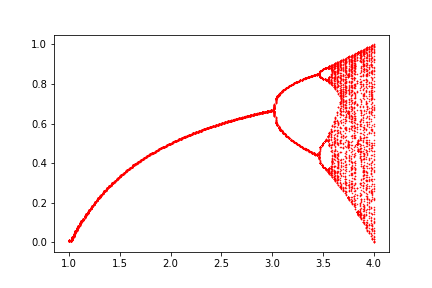
\includegraphics[scale=0.9]{../img/logistic_map_tree.png}}
\caption{Бифуркационная диаграмма логистического отображения}
\label{fig:image}
\end{figure}

\newpage

Попробуем построить предсказывающую систему, которой на вход подаётся определенное количество данных их логистического отображения, а на выходе мы получаем последующее значение в данной цепочке. После же мы сравним ляпуновские показатели изначальной системы и нейронного предсказателя. Для наших целей создадим трёхслойную нейронную сеть с заранее определенным количеством входов, с заранее определенным количеством нейронов на каждом из двух спрятанных слоёв, а также с случайно заданными весами и сдвигами для каждого из нейронов. Запуская нашу сеть, мы получаем некий результат, который, безусловно, сравниваем с желаемым результатом. Чтобы уменьшать разницу между этим двумя значениями, а именно вычисляемую среднюю квадратичную ошибку

\begin{equation*}
MSE = \dfrac{1}{n}\sum_{i=1}^{n}{(y_{true} - y_{pred})}
\end{equation*}

или, как ещё говорят, вычислим потери. 

\begin{figure}[h]
\center{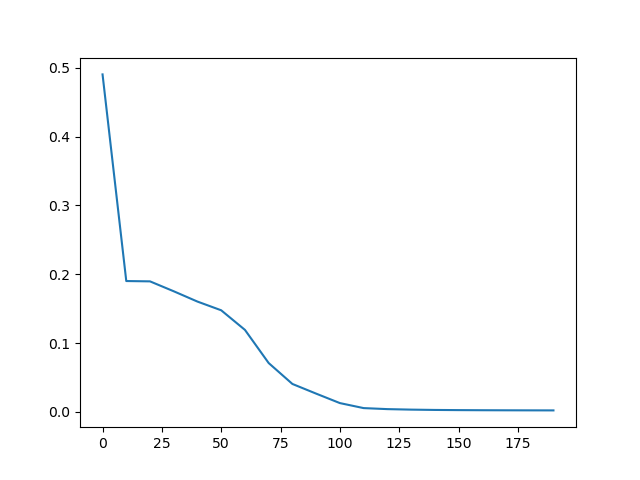
\includegraphics[scale=0.8]{../img/mse_errors.png}}
\caption{Ошибка обучения нейронной сети}
\label{fig:image}
\end{figure}

Наша функция берёт среднее значение всех ошибок, и чем меньше будет это значение, тем лучше будут предсказания. Для того, чтобы минимизировать эти потери, воспользуемся методом обратного распространения. Его суть заключается в обновлении весов и сдвигов нашего перцептрона с помощью стохастического градиентного спуска. Запишем функцию потерь как функцию от нескольких переменных:

\begin{equation*}
L(w_i, b_i),
\end{equation*}

где $w_i$ - все веса сети, а $b_i$ - все сдвиги. Рассчитаем, как изменятся потери при изменении, например, веса $w_1$:
\begin{equation*}
w_1 = w_1 - \eta \dfrac{\partial L}{\partial w_1},
\end{equation*}

где $\eta$ - скорость обучения.

Если $\dfrac{\partial L}{\partial w_1}$ положительна, то $w_1$ уменьшится, что уменьшит L. Если же $\dfrac{\partial L}{\partial w_1}$ отрицательно, то $w_1$ увеличится, что также уменьшит L. Процесс обучения таков:
\begin{itemize}
\item Выбираем одно наблюдение из набора данных. Именно то, что мы работаем только с одним наблюдением, делает наш градиентный спуск стохастическим;
\item Считаем все частные производные функции потерь по всем весам и порогам;
\item Используем формулу обновления, чтобы обновить значения каждого веса и порога;
\item Возвращаемся к первому шагу;
\end{itemize}

Данный алгоритм выполняется до тех пор, пока средняя квадратическая ошибка не будет достаточно мала. Также заранее задано количество эпох (шагов по алгоритму), чтобы в случае паралича сети задача не стала бесконечной. 

Было проведено множество испытаний, чтобы выбрать оптимальные значения входов, оптимальные значения количества нейронов на каждом из двух скрытых слоёв (так как в задании заявлена внешняя структура сети). По итогу, на вход подаётся 12 значений, а на каждом из скрытых слоёв у нас по 10 нейронов. Для обучения сети было подано 15 наборов тестовых данных, что позволило добиться достаточно быстрого снижения потерь сети. 


Для сравнения исходной системы и нейронной сети сравним ляпуновские показатели, которые помогают диагносцировать, находится ли система в хаотическом состоянии или нет. Логистическое отображение $x_{n+1} = rx_n(1-x_n)$ при значении параметра r > 3.57 становится хаотическим. При значении параметра r=4, показательно Ляпунова $\lambda = ln2 = 0.69301$. Сравним данное значение с ляпуновским показателем последовательности значений, вычисленной нейронной сетью за 40 итераций. При всех заранее объявленных параметрах сети значение показателя Ляпунова $r = 0.6825$. Погрешность для данных вычислений показателя - 0.0164. Абсолютная ошибка - 0.0106.

\section{Заключение}

По данным результатам видно, что оценка показателя Ляпунова совпадает с истинным значением показателя Ляпунова в пределах погрешности. Приложенный результат показывает, что данный метод работоспособен. В дальнейшем рассматривается возможность применения данного алгоритма для аттрактора Хенона. 
\end{document}
